\documentclass{protokol}

\usepackage[czech]{babel}
\usepackage[utf8]{inputenc}
\usepackage{icomma}

% Plovouci bloky (obrazky, tabulky)
\usepackage{floatrow}
\floatsetup[table]{capposition=top}
\floatsetup[figure]{frameset={\fboxsep16pt}}
\usepackage{subcaption}

% Tabulky
\usepackage{tabu}
\usepackage{booktabs}
\usepackage{csvsimple}
\usepackage{multirow}
\usepackage{multicol}

% Jednotky
\usepackage{siunitx}
\sisetup{
	locale               = DE,
	inter-unit-product   = \ensuremath{{}\cdot{}},
	list-units           = single,
	list-separator       = {; },
	list-final-separator = \text{ a },
	list-pair-separator  = \text{ a },
	range-phrase         = \text{ až },
	range-units          = single,
	separate-uncertainty = true,
}
\usepackage{amsmath}

% Obvody
\usepackage{circuitikz}

% Obrazky a grafy
% \usepackage{graphicx}
\graphicspath{
	{img/}
	{plots/}
	{build/plots/}
}
\usepackage{epstopdf}
\epstopdfsetup{outdir=./build/plots/}

\jmenopraktika={Experimentální metody I}       % jmeno predmetu
\jmeno={Radek Horňák, Jan Slaný, Lukáš Vrána}  % jmeno mericiho
\obor={F}                                      % zkratka studovaneho oboru
\skupina={Čt 15:00}                            % doba vyuky seminarni skupiny
\rocnik={IV}
\semestr={I}

\cisloulohy={01}
\jmenoulohy={Vektorový síťový analyzátor}

\datum={22. září 2021}                  % datum mereni ulohy
\tlak={}% [hPa]
\teplota={}% [C]
\vlhkost={}% [%]

\newcommand\sparam{S}
\newcommand\male{m}
\newcommand\female{f}
\newcommand\permitfree{\varepsilon_0}
\newcommand\permitrel{\varepsilon_r}
\newcommand\permeabfree{\mu_0}

\newcommand\connector[2]{#1 -- #2}
\newcommand\connectord[3]{#1 -- #2\\ #3}
\tikzset{
	connector/.style={
		draw,
		align=center,
		minimum width=4cm,
		minimum height=1.5cm}
}

\begin{document}
\headernoenv

\section{Úvod}
Elektrické obvody pracující na nízkých frekvencích,
jejichž rozměry jsou malé oproti vlnové délce signálu,
mají v~každém bodě jasně definované napětí a proud.
Díky malým rozměrům je v nich zároveň zanedbatelné fázové zpoždění
mezi jednotlivými body v~obvodu.
Tyto vlastnosti však obecně neplatí pro vysokofrekvenční obvody.
K~jejich analýze je potřeba přistupovat odlišným způsobem,
než jaký se využívá pro nízkofrekvenční obvody \cite{Pozar}.
V~této úloze budeme zabývat vektorovým síťovým analyzátorem,
který je vhodný pro měření parametrů vysokofrekvenčních obvodů.

\section{Teorie}

\subsection{Vektorový síťový analyzátor}

Pro označení vektorového síťového analyzátoru budeme z~anglického
vector network analyzer používat zkratku VNA.
VNA je zpravidla dvoukanálový mikrovlnný měřící přístroj,
pomocí nějž se měří rozptylové parametry elektrických obvodů
s~různými prvky pro vysokofrekvenční aplikace.
VNA je konstruován na měření velikosti a fáze prošlého a odraženého vlnění
z~měřeného obvodu,
který je obecně označován zkratkou DUT z~anglického device 
under test \cite{Pozar}.
VNA obsahuje zdroj signálu o~známých frekvencích a soustavu přijímačů,
které měří změny v~signálu způsobené připojeným DUT.
Schéma funkce přístroje je na obr.~\ref{VNA}.
Vygenerovaný signál postupuje směrem k~DUT.
Část signálu se na vstupu DUT odrazí zpět, část projde k~výstupnímu portu.
Přijímače poté porovnávají výsledný signál na ně dopadající
se signálem vygenerovaným ve zdroji.
Výsledek je poté počítačově zpracován a zobrazen na displeji.
Výstupem měření VNA jsou prvky rozptylové matice.

\begin{figure}[b]
	\centering
	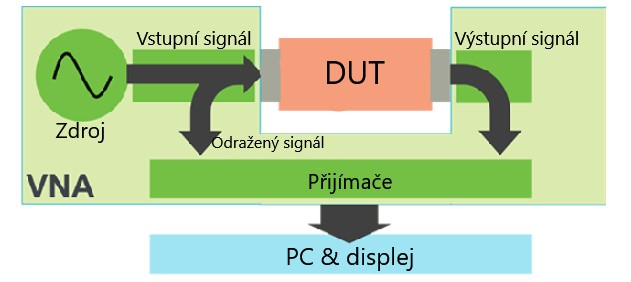
\includegraphics[width=100mm,]{network-analyzer-diagram}
	\caption{Princip funkce VNA, převzato z~\cite{schema} a upraveno}
	\label{VNA}
\end{figure}


\subsection{Rozptylová matice}

Přímé měření napětí a proudů v~mikrovlnných obvodech není vhodné,
jelikož naměřené hodnoty obsahují velikost a fázi postupující vlny
v~daném směru nebo vlny stojaté.
Je potřeba brát v~potaz dopadající, prošlé i odražené vlny.
Proto zavádíme pojem rozptylová matice, která se označuje 
jako $(S)$ matice \cite{Pozar}.
Rozptylová matice poskytuje kompletní popis obvodu s~$N$ svorkami,
konkrétně vytváří vztah mezi vlněním dopadajícím na svorky
a vlněním na svorkách odraženým.
Pro některé prvky je možné $(S)$ matice dopočítat,
ovšem jednodušší způsob je prvky matice přímo změřit pomocí VNA.
$(S)$ matice je definovaná jako:
\[
\begin{pmatrix}
	U^-
\end{pmatrix}
=
\begin{pmatrix}
	S~\end{pmatrix}
%
\begin{pmatrix}
	U^+
\end{pmatrix}
,\]
kde $U^+$ a $U^-$ jsou amplitudy dopadajícího a odraženého napětí
(v~tomto pořadí) \cite{Pozar}.

Pro obvod s~$N$ svorkami má $(S)$ matice tvar:
\[
\begin{pmatrix}
	U_1^-     \\
	U_2^-		\\
	\vdots	\\
	U_N^-
\end{pmatrix}
=
\begin{pmatrix}
	S_{11} & S_{12} & \dots & S_{1N}   \\
	S_{21} &		& 		& \vdots	\\
	\vdots &		& 		& \vdots	\\
	S_{N1} & \dots	& \dots & S_{NN} 	\\
\end{pmatrix}
%
\begin{pmatrix}
	U_1^+     \\
	U_2^+		\\
	\vdots	\\
	U_N^+
\end{pmatrix}
.\]

Pro obvod s~dvěma svorkami tedy bude $(S)$ matice řádu 2.
V~ní prvek $S_{11}$ vyjadřuje odražený signál na vstupu,
$S_{22}$ odraz na výstupu, $S_{21}$ je transmisní prvek ze vstupu na výstup
a $S_{12}$ je transmisní prvek z~výstupu na vstup.

\subsection{Impedanční a admitanční matice}

Impedance $Z$ je komplexní veličinou a je definovaná jako poměr napětí a proudu:
\begin{equation}
	Z~= \frac{U}{I} \:.
\end{equation}

Admitance $Y$ je převrácenou hodnotou impedance, tedy platí:
\begin{equation}
	Y = \frac{1}{Z} \:.
\end{equation}

Impedanční matice $(Z)$ mikrovlnného obvodu s~$N$ svorkami
udává vztah mezi napětími a proudy následovně:
\[
\begin{pmatrix}
	V_1     \\
	V_2		\\
	\vdots	\\
	V_N
\end{pmatrix}
=
\begin{pmatrix}
	Z_{11} & Z_{12} & \dots & Z_{1N}   \\
	Z_{21} &		& 		& \vdots	\\
	\vdots &		& 		& \vdots	\\
	Z_{N1} & \dots	& \dots & Z_{NN} 	\\
\end{pmatrix}
%
\begin{pmatrix}
	I_1     \\
	I_2		\\
	\vdots	\\
	I_N
\end{pmatrix}
.\]

Admitanční matice $(Y)$ je definovaná jako
\[
\begin{pmatrix}
	Y
\end{pmatrix}
=
\begin{pmatrix}
	Z~\end{pmatrix}^{-1}
,\]

což pro obvod s~$N$ svorkami můžeme rozepsat ve tvaru

\[
\begin{pmatrix}
	I_1     \\
	I_2		\\
	\vdots	\\
	I_N
\end{pmatrix}
=
\begin{pmatrix}
	Y_{11} & Y_{12} & \dots & Y_{1N}   \\
	Y_{21} &		& 		& \vdots	\\
	\vdots &		& 		& \vdots	\\
	Y_{N1} & \dots	& \dots & Y_{NN} 	\\
\end{pmatrix}
%
\begin{pmatrix}
	V_1     \\
	V_2		\\
	\vdots	\\
	V_N
\end{pmatrix}
.\]

\subsection{Výpočet impedanční a admitanční matice z~rozptylové matice}

Impedanční matici $(Z)$ můžeme vyjádřit pomocí rozptylové matice $(S)$ jako:
\[
\begin{pmatrix}
	Z~\end{pmatrix}
=
[\begin{pmatrix}
	A~\end{pmatrix}
+
\begin{pmatrix}
	S~\end{pmatrix}]
%
[\begin{pmatrix}
	A~\end{pmatrix}
-
\begin{pmatrix}
	S~\end{pmatrix}]^{-1}
,\]
kde $(A)$ je jednotková matice.
\bigskip

Obdobně můžeme pomocí rozptylové matice $(S)$ a jednotkové matice $(A)$
vyjádřit i admitanční matici jako:
\[
\begin{pmatrix}
	Y
\end{pmatrix}
=
[\begin{pmatrix}
	A~\end{pmatrix}
-
\begin{pmatrix}
	S~\end{pmatrix}]
%
[\begin{pmatrix}
	A~\end{pmatrix}
+
\begin{pmatrix}
	S~\end{pmatrix}]^{-1}
.\]

\subsection{Transmisní matice}
Při měření je v obvodu zpravidla zapojeno více prvků.
Proto je vhodné zavést transmisní matici $(T)$ pro každý z prvků.
U dvojbranů je matice $(T)$ řádu 2 a má tvar
\[
\begin{pmatrix}
	A & B  \\
	C &	D  \\
\end{pmatrix}
.\]

V nejjednodušším obvodu se dvěma prvky je mezi celkovou transmisní
maticí $(ABCD)$, transmisní maticí prvního prvku $(A_1B_1C_1D_1)$
a transmisní maticí druhého prvku $(A_2B_2C_2D_2)$ vztah následující:

\[
\begin{pmatrix}
	A & B  \\
	C &	D  \\
\end{pmatrix}
=
\begin{pmatrix}
	A_1 & B_1  \\
	C_1 & D_1  \\
\end{pmatrix}
%
\begin{pmatrix}
	A_2 & B_2  \\
	C_2 & D_2  \\
\end{pmatrix}
.\]

Dále platí:

\begin{equation}
	A = \frac{(1+S_{11})(1-S_{22})+S_{12}S_{21}}{2S_{21}},
\end{equation}

\begin{equation}
	B = Z_0 \frac{(1+S_{11})(1+S_{22})-S_{12}S_{21}}{2S_{21}},
\end{equation}

\begin{equation}
	C = \frac{1}{Z_0} \frac{(1-S_{11})(1-S_{22})-S_{12}S_{21}}{2S_{21}},
\end{equation}

\begin{equation}
	D = \frac{(1-S_{11})(1+S_{22})+S_{12}S_{21}}{2S_{21}}.
\end{equation}

Zpětný přepočet $ABCD$ prvků na $S_{11}$ a $S_{21}$ lze provést jako

\begin{equation}
	S_{11} = \frac{A+B/Z_0-CZ_0-D}{A+B/Z_0+CZ_0+D},
\end{equation}

\begin{equation}
	S_{21} = \frac{2}{A+B/Z_0+CZ_0+D}.
\end{equation}


Velikost impedance $|Z|$ určíme jako

\begin{equation}
	|Z| = Z_{11}Z_{22}-Z_{12}Z_{21},
\end{equation}

kde $Z_{11}$, $Z_{12}$, $Z_{21}$ a $Z_{22}$ jsou prvky impedanční matice, které lze pomocí prvků rozptylové matice vyjádřit jako:

\begin{equation}
	Z_{11} = Z_0 \frac{(1+S_{11})(1-S_{22})+S_{12}S_{21}}{(1-S_{11})(1-S_{22})-S_{12}S_{21}},
\end{equation}

\begin{equation}
	Z_{12} = Z_0
	\frac{2S_{12}}{(1-S_{11})(1-S_{22})-S_{12}S_{21}},
\end{equation}

\begin{equation}
	Z_{21} = Z_0
	\frac{2S_{21}}{(1-S_{11})(1-S_{22})-S_{12}S_{21}},
\end{equation}

\begin{equation}
	Z_{22} = Z_0
	\frac{(1-S_{11})(1+S_{22})+S_{12}S_{21}}{(1-S_{11})(1-S_{22})-S_{12}S_{21}}.
\end{equation}

\subsection{Typy konektorů}
V~tomto praktiku budeme měřit různá zapojení koaxiálních konektorů typu
SMA, BNC a N s~impedancí 50~$\Omega$.

SubMiniature Type-A neboli SMA konektor je jedním z~nejpoužívanějších
mikrovlnných konektorů. Je zobrazený na obr.~\ref{SMA}.
Vnitřní průměry jeho koaxiálního vedení jsou 4,1~mm a 1,27~mm,
funkci izolantu v~něm plní teflon.
Spojení se zajišťuje pomocí šroubovacího mechanismu.
Obecně se uvádí, že je vhodný až do frekvence 18~GHz \cite{rfhandbook}.

Bayonet Neill Concelman, někdy nazývaný Bayonet Navel Connector,
zkráceně BNC, je konektor vyvinutý ve čtyřicátých letech dvacátého století.
Jeho charakteristikou je bajonetový mechanismus spojení.
Tento mechanismus je tvořen dvěma výstupky na samičím konektoru
a drážkou se spirálou a vybráním na převlečné části samčího konektoru,
viz obr.~\ref{BNC}.
Umožňuje rychlé a spolehlivé spojení nasunutím a pootočením převlečné
části o~90~$^{\circ}$ \cite{czwiki}.
Konektor je vhodný až do frekvence 11~GHz \cite{rfhandbook}.

Konektor typu N, pojmenovaný po jeho vynálezci Paulu Neillovi,
vznikl ve čtyřicátých letech dvacátého století.
Jedná se o~konektor s~klasickým šroubovacím mechanismem.
Využívá se při aplikacích, kde frekvence nepřesahuje 11~GHz \cite{rfhandbook}.
Je zobrazený na obr.~\ref{N}.

\begin{center}
	\captionsetup{justification=centering}
	\begin{minipage}{0.32\textwidth}
		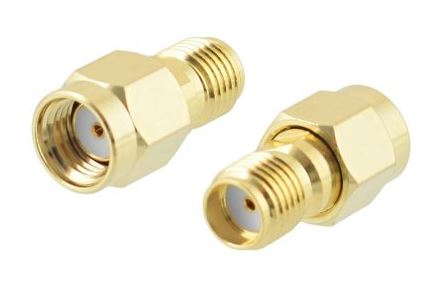
\includegraphics[width=\textwidth]{connector-sma}
		\captionof{figure}{SMA konektor, převzato z \cite{gme}}
		\label{SMA}
	\end{minipage}
	\begin{minipage}{0.40\linewidth}
		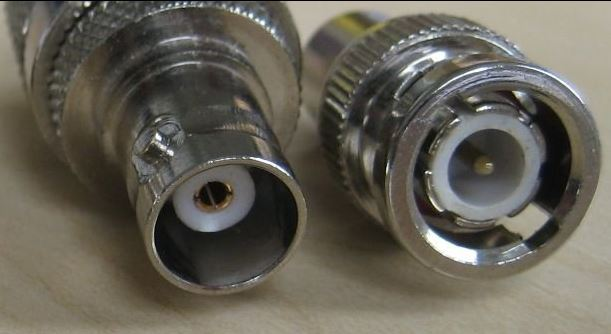
\includegraphics[width=\linewidth]{connector-bnc}
		\captionof{figure}{BNC konektor, převzato z \cite{czwiki}}
		\label{BNC}
	\end{minipage}
	\begin{minipage}{0.29\textwidth}
		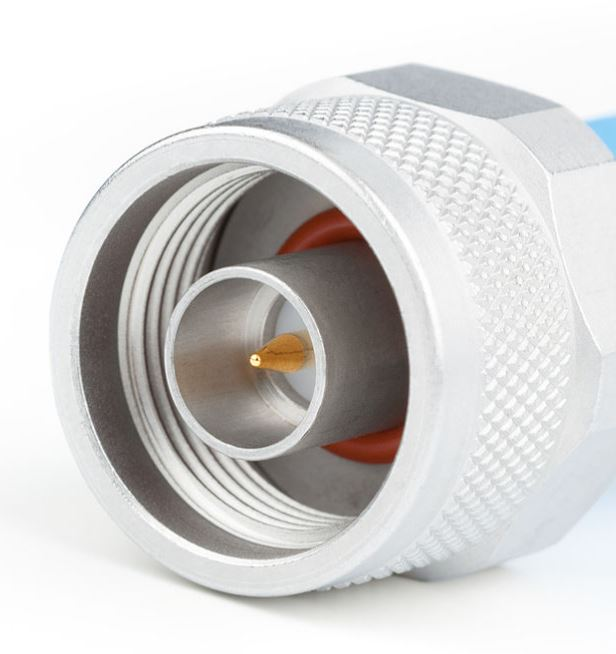
\includegraphics[width=\textwidth]{connector-n}
		\captionof{figure}{N konektor, převzato z \cite{enwiki}}
		\label{N}
	\end{minipage}
\end{center}

\section{Praktická část}
\subsection{Kalibrace přístroje}
K~měření budeme používat vektorový síťový analyzátor Rohde \& Schwarz ZVL,
který měří v~rozsahu 9~kHz až 13,6~GHz.
Měřený prvek se k~přístroji připojuje pomocí testovacích kabelů s~SMA konektory.
Tyto kabely však nejsou dokonalé a mění parametry celého systému.
Před samotným měřením je tedy potřeba přístroj s~kabely nakalibrovat.
Pro kalibraci jednoho portu potřebujeme tři různé impedance.
Z~praktických důvodů se volí známé impedance při třech situacích -- zkrat (short),
otevřený obvod (open) a přizpůsobený obvod (match).
Nejvhodnějším způsobem kalibrace je využití kalibračního členu,
pomocí nějž lze jednoduše výše zmíněné impedance vytvořit.
K~dispozici máme kalibrační člen Rohde \& Schwarz ZV-Z135,
k~němuž jsou dodávány i korekce, které už máme ve VNA nahrané.
Kalibraci je potřeba provést na každém portu zvlášť i na obou portech současně.
Zároveň je potřeba kalibraci provést pečlivě,
protože nedbalá kalibrace způsobená špatně připojeným kalibračním členem
by mohla ovlivnit všechna následně naměřená data.

První připojíme port 1 jako otevřený obvod.
Veškerý signál by se měl odrazit, čemuž odpovídá $S_{11}$ = 0~dB.
Další na řadě je zkrat na portu 1.
Na zkratu se nemá výkon kde ztratit,
takže opět dochází k~úplnému odrazu a znovu platí, že $S_{11}$ = 0~dB.
Zbývá připojení portu 1 na přizpůsobenou impedanci.
V~tomto případě by se měl ideálně veškerý signál absorbovat,
tedy $S_{11}$ by měla být co nejnižší.
U~frekvence 10~GHz je $S_{11}$ přibližně $-25$~dB,
minimum $S_{11}$ je okolo $-50$~dB. Tyto hodnoty považujeme 
za dostatečně nízké.

Kalibrace druhého portu probíhá obdobně,
přičemž se místo $S_{11}$ měří $S_{22}$.
Pro otevřený obvod, zkrat i přizpůsobený obvod dává přístroj prakticky
stejné hodnoty $S_{22}$ na portu 2 jako jsme naměřili pro $S_{11}$ na portu 1.

Posledním krokem je kalibrace obou portů současně nazývaná
jako zapojení through.
Přístroj měří $S_{21}$, která je podle očekávání kolem 0~dB.
Tím je kalibrace hotová.

Z~předpokladu symetrie budeme dále uvažovat rovnosti
$S_{11}$ = $S_{22}$ a $S_{21}$ = $S_{12}$.

\subsection{1. měření: zlatý konektor SMA\female}
Jako první měříme konektor SMA, který má z~obou stran samičí vstup (značíme f),
schéma zapojení je na obr.~\ref{fig:exp1}.
Konektor je zlaté barvy (index $_Z$), což rozlišuje pouze z důvodu,
že budeme srovnávat dva konektory stejného typu lišící se barvou.
Výsledné zapojení tedy označíme jako (SMAf/SMAf)$_Z$.
Obdobné značení budeme využívat i nadále.
Z~grafu č.~\ref{fig:01-sparam} je vidět,
že v~GHz frekvencích se na konektoru začíná signál odrážet (viz $\sparam_{11}$),
a na~frekvencích blížících se \SI{10}{\giga\hertz} je signál zeslaben téměř
o~\SI{0.5}{\decibel}.

\begin{figure}[htp]
	\centering
	\begin{circuitikz}
		\node[connector] (con1) at (0,0)
		{\connectord{SMA\female}{SMA\female}{zlatý}};
		\draw (con1.west) to[short, -o] +(-1,0);
		\draw (con1.east) to[short, -o] +(1,0);
	\end{circuitikz}
	\caption{Schéma zapojení 1. měření}
	\label{fig:exp1}
\end{figure}

\begin{figure}[htp]
	\centering
	\input{plots/data01-s11}
	\input{plots/data01-s21}
	\caption{Naměřené hodnoty parametrů $\sparam_{11}$ a~$\sparam_{21}$
		zlatého konektoru SMA\female.}
	\label{fig:01-sparam}
\end{figure}

\subsection{2. měření: stříbrný konektor SMA\female}
Měříme opět konektor (SMAf/SMAf)$_S$, avšak nyní je konektor
ve stříbrné barvě (index $_S$).
Schéma zapojení je na obr. \ref{fig:exp2}.
V porovnání s konektorem ve zlaté barvě z prvního měření
je u stříbrného z 
$S_{11}$ stříbrného konektoru na obr. \ref{fig:02-sparam} má podobný průběh jako u zlatého konektoru.
U~$S_{21}$ je vidět oproti zlatému konektoru menší útlum.
Může se tedy jednat o kvalitnější součástku,
nebo je lepší průchod signálu způsoben preciznějším dotažením.

\begin{figure}[htp]
	\centering
	\begin{circuitikz}
		\node[connector] (con1) at (0,0)
		{\connectord{SMA\female}{SMA\female}{stříbrný}};
		\draw (con1.west) to[short, -o] +(-1,0);
		\draw (con1.east) to[short, -o] +(1,0);
	\end{circuitikz}
	\caption{Schéma zapojení 2. měření}
	\label{fig:exp2}
\end{figure}

\begin{figure}[htp]
	\centering
	\input{plots/data02-s11}
	\input{plots/data02-s21}
	\caption{Naměřené hodnoty parametrů $\sparam_{11}$ a~$\sparam_{21}$
		stříbrného konektoru SMA\female.}
	\label{fig:02-sparam}
\end{figure}

\subsection{3. měření: trojice konektorů SMA}
Měříme zapojení (SMAf/SMAf)$_Z$---(SMAm/SMAm)$_Z$---(SMAf/SMAf)$_S$,
kde m značí samčí vstup.
Schéma zapojení je na obr. \ref{fig:exp3}.
Úkolem je dopočítat matice prostředního konektoru (SMAm/SMAm)$_Z$,
matice pro zbylé konektory známe z předchozích měření.

\begin{figure}[htp]
	\centering
	\begin{circuitikz}
		\node[connector] (con1) at (-4,0)
		{\connectord{SMA\female}{SMA\female}{zlatý}};
		\node[connector] (con2) at (0,0)
		{\connectord{SMA\male}{SMA\male}{zlatý}};
		\node[connector] (con3) at (4,0)
		{\connectord{SMA\female}{SMA\female}{stříbrný}};
		\draw (con1.west) to[short, -o] +(-1,0);
		\draw (con3.east) to[short, -o] +(1,0);
	\end{circuitikz}
	\caption{Schéma zapojení 3. měření}
	\label{fig:exp3}
\end{figure}

\begin{figure}[htp]
	\centering
	\input{plots/data03-s11}
	\input{plots/data03-s21}
	\caption{Naměřené hodnoty parametrů $\sparam_{11}$ a~$\sparam_{21}$
		trojice konektorů SMA.}
	\label{fig:03-sparam}
\end{figure}

\begin{figure}[htp]
	\centering
	\input{plots/results03-s11}
	\input{plots/results03-s21}
	\caption{Spočtené hodnoty parametrů $\sparam_{11}$ a~$\sparam_{21}$
		kontektoru SMA\male.}
	\label{fig:03-result-sparam}
\end{figure}

\subsection{4. měření: dvojice redukcí \connector{SMA\female}{BNC}}
Máme zapojení (SMAf/BNCm)---(BNCf/SMAf),
jeho schéma je vidět na obr.~\ref{fig:exp4}.
Jelikož nedokážeme zapojit ani jeden z těchto konektorů samostatně
a chceme znát matici jednoho z nich,
konektory budeme považovat za identické a výslednou matici
jednoho konektoru určíme jako odmocninu z naměřené matice.

\begin{figure}[htp]
	\centering
	\input{plots/data04-s11}
	\input{plots/data04-s21}
	\caption{Naměřené hodnoty parametrů $\sparam_{11}$ a~$\sparam_{21}$
		dvojice redukcí \connector{SMA\female}{BNC}.}
	\label{fig:04-sparam}
\end{figure}

\begin{figure}[htp]
	\centering
	\input{plots/results04-s11}
	\input{plots/results04-s21}
	\caption{Spočtené hodnoty parametrů $\sparam_{11}$ a~$\sparam_{21}$
		redukce \connector{SMA\female}{BNC}.}
	\label{fig:04-result-sparam}
\end{figure}

\subsection{5.měření: průchodka BNC\female}
Ze zapojení (SMAf/BNCm)---(BNCf/BNCf)---(BNCm/SMAf),
jehož schéma je vidět na obr.~\ref{fig:exp5},
chceme nalézt parametry prostředního konektoru (BNCf/BNCf).
Výpočet lze provézt díky znalosti výsledků z měření 4.

\begin{figure}[htp]
	\centering
	\input{plots/data05-s11}
	\input{plots/data05-s21}
	\caption{Naměřené hodnoty parametrů $\sparam_{11}$ a~$\sparam_{21}$
		sestavy redukcí \connector{SMA\female}{BNC} a~průchodky BNC\female.}
	\label{fig:05-sparam}
\end{figure}

\begin{figure}[htp]
	\centering
	\input{plots/results05-s11}
	\input{plots/results05-s21}
	\caption{Spočtené hodnoty parametrů $\sparam_{11}$ a~$\sparam_{21}$
		průchodky BNC\female.}
	\label{fig:05-result-sparam}
\end{figure}

\subsection{6. měření: rezonance na T-průchodce BNC}
\newcommand\freelen{d}
Zapojení (SMAf/BNCm)---(BNCf/BNCm/BNCf)---(BNCm/SMAf),
přičemž (BNCf/BNCm/BNCf) je člen ve tvaru T.
Prostřední vstup členu T je zde jako otevřený obvod, viz obr.~\ref{fig:exp6}.
Na otevřeném obvodu dochází k odrazu signálu a destruktivní interferenci.
Délka prostředního vstupu $d$ je s frekvencí $f$,
při níž dochází k destruktivní interferenci, spojena vztahem
\begin{equation}
	d = \frac{(2k+1)}{4f} \frac{1}{\sqrt{\varepsilon_0 \varepsilon_r \mu_0}},
	\label{eq:resonance-length}
\end{equation}
kde k = 0,1,2,... je řád maxima, $\varepsilon_0$ je permitivita vakua,
$\varepsilon_r = \num{2.25}$ je v tomto případě relativní permitivita polyethylenu
a $\mu_0$ je permeabilita vakua.

Pro stanovení neznámé délky $\freelen$ přepišme vztah
\eqref{eq:resonance-length} do tvaru:
\begin{align}
	\label{eq:resonance-length-freq}
	f &= \frac{1}{\freelen} \frac{2k+1}{4}
		\frac{1}{\sqrt{\permitfree\permitrel\permeabfree}}
		= ax + b &
	a &= 1/\freelen \\
	& &
	x &= \frac{2k+1}{4}
		\frac{1}{\sqrt{\permitfree\permitrel\permeabfree}}
\end{align}
kde parametry $a$ a $b$ aproximujeme metodou nejmenších čtverců
a~spočteme délku $\freelen = 1/a$.

Destruktivní interference pro $\lambda/4$ nastává při frekvenci 3,33~GHz
s~útlumem 42~dB. Pro $3\lambda/4$ je útlum 36,4~dB na
frekvenci 8,47~GHz.
Délka $d$ spočtená podle vztahu~\eqref{eq:resonance-length-freq} je
\SI{19.4}{\milli\metre}.
% TODO: Calculate uncertainty

\begin{figure}[htp]
	\centering
	\begin{circuitikz}
		\node[connector, minimum height=1.5cm] (con1) at (-4,0)
		{\connector{SMA\female}{BNC\male}};
		\draw (-2,-0.75) -- (2,-0.75) -- (2,0.75) -- (0.75,0.75) -- (0.75,2)
		-- (-0.75,2) -- (-0.75,0.75) -- (-2,0.75) -- cycle;
		\node at (-1.2,0) {BNC\female};
		\node at (0,1.375) {BNC\male};
		\node at (1.2,0) {BNC\female};
		\node[connector, minimum height=1.5cm] (con3) at (4,0)
		{\connector{BNC\male}{SMA\female}};
		\draw (con1.west) to[short, -o] +(-1,0);
		\draw (con3.east) to[short, -o] +(1,0);
	\end{circuitikz}
	\caption{Schéma zapojení 6. měření}
	\label{fig:exp6}
\end{figure}

\begin{figure}[htp]
	\centering
	\input{plots/data06-s11}
	\input{plots/data06-s21}
	\caption{Naměřené hodnoty parametrů $\sparam_{11}$ a~$\sparam_{21}$
		sestavy redukcí \connector{SMA\female}{BNC} a~T-průchodky BNC.}
	\label{fig:06-sparam}
\end{figure}

\subsection{7. měření: rezonance na T-průchodce s volným vodičem}
Měříme (SMAf/BNCm)---(BNCf/BNCm + kabel /BNCf)---(BNCm/SMAf).
Zapojení je stejné jako u měření 6, tentokrát je však na prostřední vstup
T členu připojen kabel neznámé délky. %Mění se fáze?

Postup je obdobný předchozímu případu. Pro výpočet déllky $\freelen$
jsme zvolili minima signálu $\sparam_{21}$ příslušící frekvencím
pod \SI{3e8}{\hertz}, tedy patnáct hodnot.
U~vyšších frekvencí roste nejistota určení polohy minima, jelikož
se prodlužuje krok vzorkování, a proto nebyly uvažovány.

Délka kabelu spočtená výše uvedenou metodou činí
$\freelen = \SI{5.072(4)}{\metre}$.

\begin{figure}[htp]
	\centering
	\begin{circuitikz}
		\node[connector, minimum height=1.5cm] (con1) at (-4,0)
		{\connector{SMA\female}{BNC\male}};
		\draw (-2,-0.75) -- (2,-0.75) -- (2,0.75) -- (0.75,0.75) -- (0.75,2)
		-- (-0.75,2) -- (-0.75,0.75) -- (-2,0.75) -- cycle;
		\node at (-1.2,0) {BNC\female};
		\node at (0,1.375) {BNC\male};
		\node at (1.2,0) {BNC\female};
		\node[connector, minimum height=1.5cm] (con3) at (4,0)
		{\connector{BNC\male}{SMA\female}};
		\draw (0,2) to[short, -o] (0,3);
		\draw (con1.west) to[short, -o] +(-1,0);
		\draw (con3.east) to[short, -o] +(1,0);
	\end{circuitikz}
	\caption{Schéma zapojení 7. měření}
	\label{fig:exp7}
\end{figure}

\begin{figure}[htp]
	\centering
	\input{plots/data07-s11}
	\input{plots/data07-s21}
	\caption{Naměřené hodnoty parametrů $\sparam_{11}$ a~$\sparam_{21}$
		sestavy redukcí \connector{SMA\female}{BNC}
		a~T-průchodky BNC s volným vodičem.}
	\label{fig:07-sparam}
\end{figure}

\subsection{8. měření: rezonance na T-průchodce s~vodičem zakončeným terminátorem}
Zapojení (SMAf/BNCm)---(BNCf/BNCm + kabel + terminátor /BNCf)---(BNCm/SMAf)
vychází z měření 7, ke kabelu je navíc připojen terminátor.

\begin{figure}[htp]
	\centering
	\input{plots/data08-s11}
	\input{plots/data08-s21}
	\caption{Naměřené hodnoty parametrů $\sparam_{11}$ a~$\sparam_{21}$
		sestavy redukcí \connector{SMA\female}{BNC}
		a~T-průchodky BNC s~vodičem a~terminátorem.}
	\label{fig:08-sparam}
\end{figure}

\subsection{9. měření: banánkový spoj}
Zapojení (SMAf/BNCm)---(BNCf/banánky m)---(banánky f/BNCf)---(BNCm/SMAf),
přičemž ba\-nán\-ky je koaxiální vedení zapojeno způsobem
jádro--jádro a stínění--stínění.

\begin{figure}[htp]
	\centering
	\begin{circuitikz}
		\node[connector] (con1) at (-5,0)
		{\connector{SMA\female}{BNC\male}};
		\node[connector, minimum width=1.4cm] (con2) at (-2.3,0)
		{BNC\female};
		\node[connector, minimum width=1.4cm] (con3) at (2.3,0)
		{BNC\female};
		\coordinate[yshift=2mm] (n1) at (con2.east) {};
		\coordinate[yshift=0-2mm] (n2) at (con2.east) {};
		\coordinate[yshift=2mm] (n3) at (con3.west) {};
		\coordinate[yshift=0-2mm] (n4) at (con3.west) {};
		\draw (n1) to[short, -o] +(1.4,0);
		\draw (n2) to[short, -*] +(1.4,0);
		\draw (n3) to[short, -o] +(-1.4,0);
		\draw (n4) to[short, -*] +(-1.4,0);
		\node at (0,0.6) {banánky};
		\node[connector] (con4) at (5,0)
		{\connector{BNC\male}{SMA\female}};
		\draw (con1.west) to[short, -o] +(-1,0);
		\draw (con4.east) to[short, -o] +(1,0);
	\end{circuitikz}
	\caption{Schéma zapojení 9. měření}
	\label{fig:exp9}
\end{figure}

\begin{figure}[htp]
	\centering
	\input{plots/data09-s11}
	\input{plots/data09-s21}
	\caption{Naměřené hodnoty parametrů $\sparam_{11}$ a~$\sparam_{21}$
		sestavy redukcí \connector{SMA\female}{BNC}
		a~\connector{BNC}{banánky}.}
	\label{fig:09-sparam}
\end{figure}

\subsection{10. měření}
Vycházíme ze zapojení jako u měření 9
(SMAf/BNCm)---(BNCf/banánky m)---(banánky f/BNCf)---(BNCm/SMAf),
přičemž nyní přehozením banánků máme zapojení koaxiálního vedení do kříže,
tedy jádro--stínění.

Podle očekávání dostáváme horší výsledky než v měření 9....

\begin{figure}[htp]
	\centering
	\begin{circuitikz}
		\node[connector] (con1) at (-5,0)
		{\connector{SMA\female}{BNC\male}};
		\node[connector, minimum width=1.4cm] (con2) at (-2.3,0)
		{BNC\female};
		\node[connector, minimum width=1.4cm] (con3) at (2.3,0)
		{BNC\female};
		\coordinate[yshift=2mm] (n1) at (con2.east) {};
		\coordinate[yshift=0-2mm] (n2) at (con2.east) {};
		\coordinate[yshift=2mm] (n3) at (con3.west) {};
		\coordinate[yshift=0-2mm] (n4) at (con3.west) {};
		\draw (n1) to[short, -o] +(1.4,0);
		\draw (n2) to[short, -*] +(1.4,0);
		\draw (n3) to[short, -*] +(-1.4,0);
		\draw (n4) to[short, -o] +(-1.4,0);
		\node at (0,0.6) {banánky};
		\node[connector] (con4) at (5,0)
		{\connector{BNC\male}{SMA\female}};
		\draw (con1.west) to[short, -o] +(-1,0);
		\draw (con4.east) to[short, -o] +(1,0);
	\end{circuitikz}
	\caption{Schéma zapojení 10. měření}
	\label{fig:exp10}
\end{figure}

\begin{figure}[htp]
	\centering
	\input{plots/data10-s11}
	\caption{$s_{11}$}
	\label{fig:10-s11}
\end{figure}

\begin{figure}[htp]
	\centering
	\input{plots/data10-s21}
	\caption{$s_{21}$}
	\label{fig:10-s21}
\end{figure}

\subsection{11. měření}
Zapojení (SMAf/BNCm)---(BNCf/banánky m)---(krokodýlky na prázdno)
jako jednobran bez připojeného přijímače.

\begin{figure}[htp]
	\centering
	\input{plots/data11-s11}
	\caption{$s_{11}$}
	\label{fig:11-s11}
\end{figure}

\subsection{12. měření}
Zapojení (SMAf/BNCm)---(BNCf/banánky m)---(krokodýlky + cívka) jako jednobran.

\begin{figure}[htp]
	\centering
	\begin{circuitikz}
		\node[connector] (con1) at (-5,0)
		{\connector{SMA\female}{BNC\male}};
		\node[connector, minimum width=1.4cm] (con2) at (-2.3,0)
		{BNC\female};
		\coordinate[yshift=0-2mm] (n2) at (con2.east) {};
		\draw (con2.east)++(0,0.2) to[short, -o] ++(1.4,0) -- ++(0,0.5)
		-- node[midway] (clip1) {} ++(4,0) to[inductor]
		++(0,-1.4) -- node[midway] (clip2) {} ++(-4,0) -- ++(0,0.5);
		\draw (con2.east)++(0,-0.2) to[short, -*] +(1.4,0);
		\draw[very thick] (clip1.center) -- +(150:1);
		\draw (clip1.center) +(-0.7,0) arc (180:150:0.7);
		\draw[very thick] (clip2.center) -- +(150:1);
		\draw (clip2.center) +(-0.7,0) arc (180:150:0.7);
		\node[yshift=1cm] at (clip2) {krokodýlky};
		\draw (con1.west) to[short, -o] +(-1,0);
	\end{circuitikz}
	\caption{Schéma zapojení 12. měření}
	\label{fig:exp12}
\end{figure}

\begin{figure}[htp]
	\centering
	\input{plots/data12-s11}
	\caption{$s_{11}$}
	\label{fig:12-s11}
\end{figure}


\subsection{13. měření}
(SMAf/BNCm)---(BNCf/banánky m)---(krokodýlky s kondenzátorem)

\begin{figure}[htp]
	\centering
	\input{plots/data13-s11}
	\caption{$s_{11}$}
	\label{fig:13-s11}
\end{figure}

\subsection{14. měření}
(SMAf/BNCf)---(BNCm/kabel/banánky)

\begin{figure}[htp]
	\centering
	\input{plots/data14-s11}
	\caption{$s_{11}$}
	\label{fig:14-s11}
\end{figure}

\subsection{15. měření}
(SMAf/BNCf)---(BNCm/kabel/banánky)---(rezistor)

\begin{figure}[htp]
	\centering
	\input{plots/data15-s11}
	\caption{$s_{11}$}
	\label{fig:15-s11}
\end{figure}

\subsection{16. měření}
(SMAf/BNCf)---(BNCm/terminátor)

\begin{figure}[htp]
	\centering
	\input{plots/data16-s11}
	\caption{$s_{11}$}
	\label{fig:16-s11}
\end{figure}

\subsection{17. měření}
(SMAf/SMAf)---(vlnovod)---(SMAm/SMAm)

\begin{figure}[htp]
	\centering
	\input{plots/data17-s21}
	\caption{$s_{21}$}
	\label{fig:17-s21}
\end{figure}

\newpage
\begin{thebibliography}{}

	\bibitem{Pozar}
	Pozar, David M. Microwave Engineering. 2012. ISBN 9781118213636

	\bibitem{schema}
	https://uk.tek.com/

	\bibitem{rfhandbook}
	Belov, L. A., et al. Handbook of RF, Microwave, and Millimeter-Wave Components. Artech House, 2012.

	\bibitem{czwiki}
	https://cs.wikipedia.org/

	\bibitem{gme}
	https://gme.cz/

	\bibitem{enwiki}
	ttps://en.wikipedia.org/

\end{thebibliography}

\end{document}
